\documentclass[11pt,a4paper,titlepage]{article}
\usepackage[a4paper]{geometry}
\usepackage[utf8]{inputenc}
\usepackage[english]{babel}
\usepackage{lipsum}

\usepackage{amsmath, amssymb, amsfonts, amsthm}
\usepackage{microtype}

\usepackage{graphicx}
\graphicspath{ {./pics/} {./eps/} {./png/}}
\usepackage{epsfig}
\usepackage{epstopdf}

\usepackage[svgnames]{xcolor}

\definecolor{MyColor1}{rgb}{0.2,0.4,0.6}
\newcommand{\textb}{\color{Black} \usefont{OT1}{lmss}{m}{n}}
\newcommand{\blue}{\color{MyColor1} \usefont{OT1}{lmss}{m}{n}}
\newcommand{\blueb}{\color{MyColor1} \usefont{OT1}{lmss}{b}{n}}
\newcommand{\red}{\color{LightCoral} \usefont{OT1}{lmss}{m}{n}}
\newcommand{\green}{\color{Turquoise} \usefont{OT1}{lmss}{m}{n}}

\usepackage{titlesec}
\usepackage{sectsty}

\sectionfont{\color{MyColor1}}
\subsectionfont{\color{MyColor1}}

\usepackage{caption}
\usepackage[american, smartlabels]{circuitikz}

\makeatletter
\let\reftagform@=\tagform@
\def\tagform@#1{\maketag@@@{(\ignorespaces\textcolor{red}{#1}\unskip\@@italiccorr)}}
\renewcommand{\eqref}[1]{\textup{\reftagform@{\ref{#1}}}}
\makeatother
\usepackage{hyperref}
\hypersetup{colorlinks=true}

\title{\Huge \blueb Dawn of Empires \\ \vspace{10mm}
  \blue Game rules}
\date{}

\begin{document}
\maketitle

\section{Contents}{
  \begin{itemize}
  \item Game board
  \item 25 terrain tiles (6 ocean, 4 grassland, 4 plains, 4 forest, 3 hills, 3 mountains, 1 desert)
  \item 25 terrain cubes (one for each terrain tile)
  \item 48 technology tiles
  \item 25 city improvement tiles
  \item 9 wonder tiles
  \item For each of the 4 players:
    \begin{itemize}
    \item 1 player board
    \item 9 huts
    \item 8 warriors
    \item 2 settlers
    \item 6 resource markers (food, production, wealth, money, science, military experience)
    \item 1 rondel marker
    \end{itemize}
  \end{itemize}
}\label{sec:contents}

\section{Summary}{
  Your goal is to be the most successful empire, which is measured by
  victory points. Victory points can be gained by building and growing towns,
  researching technological advances and building wonders. Victory points
  can also be obtained from battles through military experience and by
  converting slain warriors into legends in victorious battles.
}\label{sec:summary}

\section{Game preparation}{
  Randomize the player order. Then in reverse player order, each player
  chooses an empire to play with, takes the corresponding player board, takes
  the required initial terrain tiles and places those tiles in any of the
  available starting positions. All the remaining terrain tiles are shuffled
  and placed face down as unexplored tiles in the areas between starting
  positions, as shown in the following example figures.

  \begin{figure}[!htb]
    \begin{minipage}[c]{0.4\textwidth}
      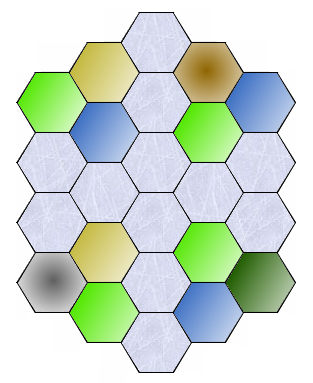
\includegraphics[scale=.5]{doe_4p_setup.png}
      \captionsetup{labelformat=empty}
      \caption{4 players}
    \end{minipage}\hfill
    \begin{minipage}[c]{0.4\textwidth}
      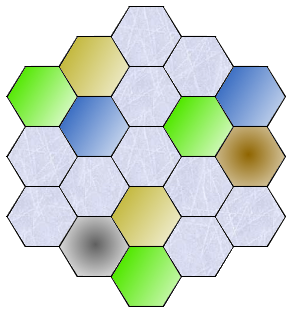
\includegraphics[scale=.5]{doe_3p_setup.png}
      \captionsetup{labelformat=empty}
      \caption{3 players}
    \end{minipage}\hfill
    \begin{minipage}[c]{0.2\textwidth}
      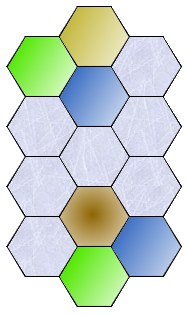
\includegraphics[scale=.5]{doe_2p_setup.png}
      \captionsetup{labelformat=empty}
      \caption{2 players}
    \end{minipage}\hfill
    \label{fig:tech_sailing}
  \end{figure}

  Then each player places resource markers to 0 in all 6 resource tracks
  (food, production, wealth, money, science, military experience).
  Place all 9 huts on town upkeep track and move the leftmost of them
  to the middle of your three starting tiles.
  Place the 7 warriors on military upkeep track
  and finally place the rondel marker to the middle of the rondel. On the
  first turn you may freely select any of the rondel spaces.

  Place all wonder tiles on the game board in appropriate places and sort
  the technology and city improvement tiles and place them near the game
  board so all players can reach them.
}\label{sec:preparation}

\section{Player turn}{
  On your turn you must move the rondel marker up to 2 spaces on the rondel
  and then you may perform the corresponding action. If a rondel space contains
  two possible actions, you can only select one of them. The possible actions
  are:
  \begin{itemize}
  \item Harvest
  \item Research
  \item Recruit
  \item Move
  \item Explore
  \item Build
  \item Grow
  \end{itemize}

  \noindent
  If you have Code of Laws technology, you may move the rondel marker up to
  3 spaces on the rondel. If you have Monarchy technology, you may move the
  rondel marker an arbitrary number of extra steps, but each extra step costs
  1 money.

  \subsection{Harvest}{
    Harvest action consists of 4 parts:
    \begin{itemize}
    \item Collect cubes
    \item Check happiness
    \item Convert cubes
    \item Pay upkeep
    \end{itemize}

    \subsubsection{Collect cubes}{
      Each town (located in tile corners) can collect up to its size terrain
      cubes from its 3 adjacent terrain tiles. If a terrain tile is occupied
      by a unit, only that player is allowed to collect the cube. Otherwise
      only players whose sum of town sizes around the tile is the highest
      (including ties) may collect the cube.

      \begin{figure}[!htb]
        \begin{minipage}[c]{0.2\textwidth}
          \label{fig:tech_irrigation}
          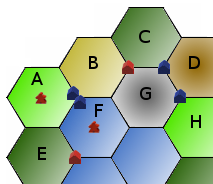
\includegraphics[scale=.6]{doe_example_cube_collection.png}
        \end{minipage}\hfill
        \begin{minipage}[c]{0.4\textwidth}
          \captionsetup{labelformat=empty, justification=justified, singlelinecheck=false}
          \caption{Example: Red player may collect cubes from tiles C, E and F.
            Blue player may collect from tiles B, C, D, G and H.}
        \end{minipage}\hfill
        \label{fig:example_cube_collection}
      \end{figure}
    }\label{subsubsec:collect_cubes}

    \subsubsection{Check happiness}{
      Once cubes are collected, you should take a look at the unhappy faces
      on your town upkeep track. You lose 1 cube of your choice for each
      revealed unhappy face which is not canceled with a happy face. You may
      gain happy faces from technologies, city improvements and wonders.
    }\label{subsubsec:check_happiness}

    \subsubsection{Convert cubes}{
      After checking happiness, you must convert the cubes to basic resources
      (food, production and wealth) and return the cubes back to the map.
      Green technologies and some of the wonders may bring new, better conversion
      ratios which can also be used. Note the the maximum amount for resources
      on the player board. If you would get more from a conversion, the leftover
      is wasted.

      While doing the conversions, you may convert wealth to money or science
      and you should usually do so, because at the end of Harvest wealth drops
      back to 0 unless you have the city improvement Court.
    }\label{subsubsec:convert_cubes}

    \subsubsection{Pay upkeep}{
      Finally, you should pay the town and military upkeep. If you cannot pay,
      you have to remove huts and warriors from the board to the upkeep track
      (filling it from right to left) until the upkeep can be paid.
    }\label{subsubsec:pay_upkeep}

  }\label{subsec:harvest}
  \subsection{Research}{
    Pick one of the available technologies from the pool, pay its cost
    in science and place it on your player board in appropriate place. You
    may not research the same technology multiple times and you may only
    research up to 3 technologies of the same color.
  }\label{subsec:research}
  \subsection{Recruit}{
    First pay 1 production. Then choose one of the tiles adjacent to your
    towns and either place the leftmost warrior from military upkeep track
    or a settler from the player board to that tile. If you decide to recruit
    a settler, you also have to pay the additional cost printed on the player
    board (usually 2 food). After recruiting, a combat may occur if the tile
    contains rival units (see Combat section).

    Alternatively, if your warrior has been enslaved by an opponent, you may
    give the paid 1 production to that player to release the warrior. In that
    case the warrior is moved back from opponent's military upkeep track to
    your own.

    If you have city improvement Barracks, you may recruit an additional
    warrior during the same action by paying 1 production, but you may not
    free two enslaved warriors or recruit two settlers with Barracks.
  }\label{subsec:recruit}
  \subsection{Move}{
    Choose a stack, which may consist of any number of warriors and settlers
    in one location. You then have the following options:
    \begin{itemize}
    \item Move the stack to an adjacent tile and resolve combat if it occurs
      (see Combat section)
    \item Raid an adjacent rival town (see Raid section)
    \item If the stack contains a settler, exchange it for a town of size 1
      in an adjacent empty corner, which must have 3 adjacent terrain tiles
      and at least 1 of them must be non-ocean tile. Place the settler back
      to the player board and take the leftmost hut from town upkeep track.
    \end{itemize}

    \begin{figure}[!htb]
      \begin{minipage}[c]{0.2\textwidth}
        \label{fig:tech_irrigation}
        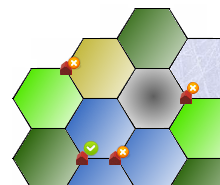
\includegraphics[scale=.6]{doe_example_new_town.png}
      \end{minipage}\hfill
      \begin{minipage}[c]{0.4\textwidth}
        \captionsetup{labelformat=empty, justification=justified, singlelinecheck=false}
        \caption{Example: It is not allowed to found new towns on the edge
          of the map or in middle of 3 ocean tiles.}
      \end{minipage}\hfill
      \label{fig:example_new_town}
    \end{figure}
    
    \noindent
    Note that you are not allowed to move to ocean tiles unless you have
    researched Sailing technology. There are also two other red technologies
    which affect the movement, but neither can be used to raid or found a town
    more than once. Horseback Riding lets you move the same stack twice, but
    cannot be used if the first move target is mountain, ocean or occupied
    by an enemy. Military tactics lets you move two different stacks. The two
    technologies work together so you are allowed to move two stacks twice, but
    the limitation of at most 1 raid or new town still applies.
    
  }\label{subsec:move}
  \subsection{Explore}{
    Choose any unexplored tile which is adjacent to any of your warriors and
    turn it around. Then you immediately get the exploration bonus, which is
    printed on the tile.
  }\label{subsec:explore}
  \subsection{Build}{
    Pick one of the city improvements or wonders and pay its cost in production
    and money. City improvements should be placed on your player board and
    wonders next to the board. You are not allowed to build the same city
    improvement multiple times. Building always requires some technology so
    before building, ensure that you have already researched the required
    technology.

    \begin{figure}[!htb]
      \begin{minipage}[c]{0.2\textwidth}
        \label{fig:tech_irrigation}
        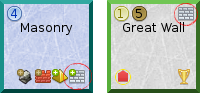
\includegraphics[scale=.6]{doe_example_build.png}
      \end{minipage}\hfill
      \begin{minipage}[c]{0.55\textwidth}
        \captionsetup{labelformat=empty, justification=justified, singlelinecheck=false}
        \caption{Example: You need Masonry technology to build Great Wall and you need to pay 1 money and 5 production.}
      \end{minipage}\hfill
      \label{fig:example_towns}
    \end{figure}

  }\label{subsec:build}
  \subsection{Grow}{
    Pay the growth cost printed on your player board (usually 4 food) and
    increase the size of one of your towns by 1 by adding the leftmost hut
    from town upkeep track to the same corner.
    \begin{figure}[!htb]
      \begin{minipage}[c]{0.2\textwidth}
        \label{fig:tech_irrigation}
        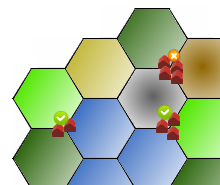
\includegraphics[scale=.6]{doe_example_grow.png}
      \end{minipage}\hfill
      \begin{minipage}[c]{0.4\textwidth}
        \captionsetup{labelformat=empty, justification=justified, singlelinecheck=false}
        \caption{Example: It is not allowed to grow a town beyond size 3.}
      \end{minipage}\hfill
      \label{fig:example_grow}
    \end{figure}
  }\label{subsec:grow}
}\label{sec:player_turn}

\section{Combat}{
  Combat may occur in two cases: By recruiting or moving a stack to a tile
  which is occupied by an enemy. In both cases active player is the attacker.
  If two rival warriors end up in the same location, both of them are killed.
  If a warrior encounters a rival settler which is not guarded by any warriors,
  the settler is killed. If two rival settlers end up in the same location,
  both of them are killed. If the attacker has Iron Working technology, the
  opponent unit will die first instead of both units dying at the same time.

  Whenever a warrior is killed, it's returned to the military upkeep track.
  If a settler is killed, it's returned to the player board. For each killed
  rival warrior you gain 1 experience point, which is measured in a separate
  experience track. At the end of the game you gain 1 victory point for each
  player who has less experience than you.

  \subsection{Legends}{
    If you win the combat, but lose at least 1 warrior you have the option to
    promote one of the dead warriors to a legend instead of returning it to
    military upkeep track. Each legend is worth 1 victory point at the end of
    the game. If you run out of money during paying the upkeep when doing the
    Harvest action you are allowed but not forced to return legends to warrior
    upkeep track instead of returning warriors from the map until you have
    enough money to pay the upkeep.
  }\label{subsec:legends}

  \subsection{Spirit of Mars}{
    If the white warrior (Spirit of Mars) is included in a combat, it is always
    the last warrior to die, but if it dies, the owner of the wonder Temple of
    Mars may immediately place it back in a non-hostile tile adjacent to any
    of his towns. If such tiles do not exist, Spirit of Mars frowns upon the
    player and is removed from the game. You gain military experience normally
    from killing the Spirit of Mars.
  }\label{subsec:spirit_of_mars}
  
  \subsection{Raid}{
    During movement, you may have the option to raid enemy towns. If you
    decide to do so, return 1 warrior from the chosen stack to your military
    upkeep track and then you can choose to either plunder or enslave:

    \begin{itemize}
      \item Plunder: take up to 2 food, 2 production, 2 money or 2 science
        from the opponent.
      \item Enslave: take 1 enemy warrior from his military upkeep track to
        yours if the opponent military upkeep track is not empty.
    \end{itemize}

    \noindent
    If the opponent has city improvement Walls, you need a stack of two
    warriors or more in order to plunder or enslave, but you still only lose
    only 1 of them in the raid. If the opponent has wonder Great Wall, you
    cannot raid him at all.
  }\label{subsec:raid}
}\label{sec:combat}
\section{End of the game}{
  Players keep taking actions like explained above until one of the following
  conditions is met:
  \begin{itemize}
  \item One of the players has built all of his huts
  \item One of the players has researched 12 technologies
  \item One of the players has 20 military experience or more
  \end{itemize}

  \noindent
  Then, each player gets one more turn, including the player who triggered the
  game end and after that victory points are calculated:
  \begin{itemize}
  \item Each hut is worth 1 point
  \item Each technology is worth 1 point
  \item Each legend is worth 1 point
  \item City improvement Palace is worth 1 point
  \item Wonders provide victory points according to the text
  \item For each player who is below you in military experience gain 1 victory point
  \end{itemize}
}\label{sec:game_end}

\newpage
\section{Appendix: Game board}{
  \begin{figure}[!htb]
    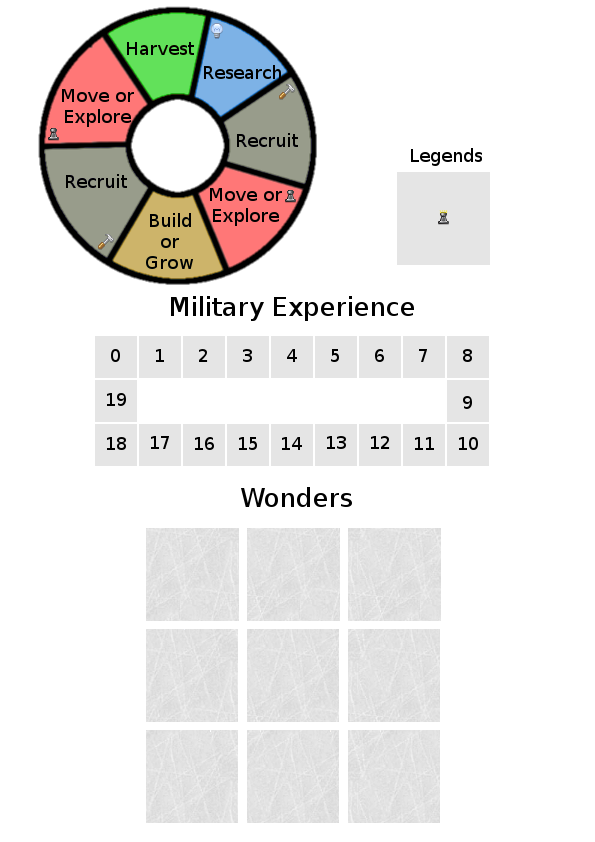
\includegraphics[scale=.6]{doe_central_board.png}
    \captionsetup{labelformat=empty}
    \caption{}
    \label{fig:game_board}
  \end{figure}
}\label{sec:game_board}

\newpage
\section{Appendix: Player board}{
  \begin{figure}[!htb]
    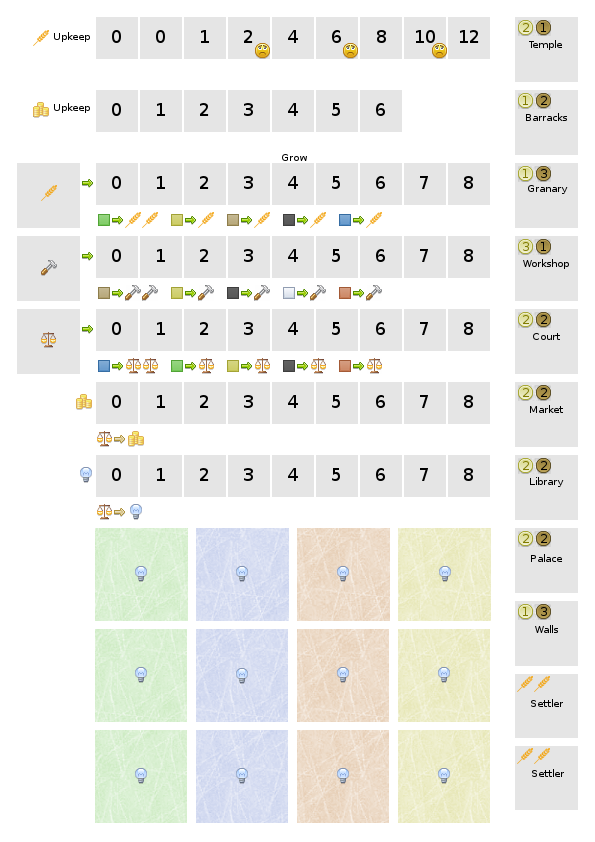
\includegraphics[scale=.6]{doe_player_board.png}
    \captionsetup{labelformat=empty}
    \caption{}
    \label{fig:game_board}
  \end{figure}
}\label{sec:player_board}

\newpage
\section{Appendix: Technology tiles}{
  \subsection{Green technologies}{

  \begin{figure}[!htb]
    \begin{minipage}[c]{0.1\textwidth}
      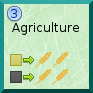
\includegraphics[scale=.7]{doe_tech_agriculture.png}
    \end{minipage}\hfill
    \begin{minipage}[c]{0.6\textwidth}
      \captionsetup{labelformat=empty, justification=justified, singlelinecheck=false}
      \caption{During harvest, you may convert cubes from plains or hills to 2 food each. (1)}
    \end{minipage}\hfill
    \label{fig:tech_agriculture}
  \end{figure}

  \begin{figure}[!htb]
    \begin{minipage}[c]{0.1\textwidth}
      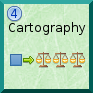
\includegraphics[scale=.7]{doe_tech_cartography.png}
    \end{minipage}\hfill
    \begin{minipage}[c]{0.6\textwidth}
      \captionsetup{labelformat=empty, justification=justified, singlelinecheck=false}
      \caption{During harvest, you may convert cubes from ocean to 3 wealth each. (1)}
    \end{minipage}\hfill
    \label{fig:tech_cartography}
  \end{figure}

  \begin{figure}[!htb]
    \begin{minipage}[c]{0.1\textwidth}
      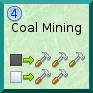
\includegraphics[scale=.7]{doe_tech_coal_mining.png}
    \end{minipage}\hfill
    \begin{minipage}[c]{0.6\textwidth}
      \captionsetup{labelformat=empty, justification=justified, singlelinecheck=false}
      \caption{During harvest, you may convert cubes from hills to 3 production each or cubes from mountains to 2 production each. (1)}
    \end{minipage}\hfill
    \label{fig:tech_coal_mining}
  \end{figure}

  \begin{figure}[!htb]
    \begin{minipage}[c]{0.1\textwidth}
      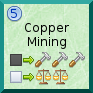
\includegraphics[scale=.7]{doe_tech_copper_mining.png}
    \end{minipage}\hfill
    \begin{minipage}[c]{0.6\textwidth}
      \captionsetup{labelformat=empty, justification=justified, singlelinecheck=false}
      \caption{During harvest, you may convert cubes from hills to 3 production each or cubes from mountains to 2 wealth each. (1)}
    \end{minipage}\hfill
    \label{fig:tech_copper_mining}
  \end{figure}

  \begin{figure}[!htb]
    \begin{minipage}[c]{0.1\textwidth}
      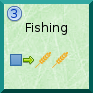
\includegraphics[scale=.7]{doe_tech_fishing.png}
    \end{minipage}\hfill
    \begin{minipage}[c]{0.6\textwidth}
      \captionsetup{labelformat=empty, justification=justified, singlelinecheck=false}
      \caption{During harvest, you may convert cubes from ocean to 2 food each. (2)}
    \end{minipage}\hfill
    \label{fig:tech_fishing}
  \end{figure}

  \begin{figure}[!htb]
    \begin{minipage}[c]{0.1\textwidth}
      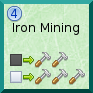
\includegraphics[scale=.7]{doe_tech_iron_mining.png}
    \end{minipage}\hfill
    \begin{minipage}[c]{0.6\textwidth}
      \captionsetup{labelformat=empty, justification=justified, singlelinecheck=false}
      \caption{During harvest, you may convert cubes from hills to 2 production each or cubes from mountains to 3 production each. (1)}
    \end{minipage}\hfill
    \label{fig:tech_iron_mining}
  \end{figure}

  \begin{figure}[!htb]
    \begin{minipage}[c]{0.1\textwidth}
      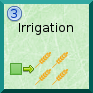
\includegraphics[scale=.7]{doe_tech_irrigation.png}
    \end{minipage}\hfill
    \begin{minipage}[c]{0.6\textwidth}
      \captionsetup{labelformat=empty, justification=justified, singlelinecheck=false}
      \caption{During harvest, you may convert cubes from grassland to 3 food each. (2)}
    \end{minipage}\hfill
    \label{fig:tech_irrigation}
  \end{figure}

  \begin{figure}[!htb]
    \begin{minipage}[c]{0.1\textwidth}
      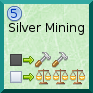
\includegraphics[scale=.7]{doe_tech_silver_mining.png}
    \end{minipage}\hfill
    \begin{minipage}[c]{0.6\textwidth}
      \captionsetup{labelformat=empty, justification=justified, singlelinecheck=false}
      \caption{During harvest, you may convert cubes from hills to 2 production each or cubes from mountains to 3 wealth each. (1)}
    \end{minipage}\hfill
    \label{fig:tech_silver_mining}
  \end{figure}

  \begin{figure}[!htb]
    \begin{minipage}[c]{0.1\textwidth}
      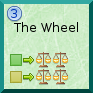
\includegraphics[scale=.7]{doe_tech_wheel.png}
    \end{minipage}\hfill
    \begin{minipage}[c]{0.6\textwidth}
      \captionsetup{labelformat=empty, justification=justified, singlelinecheck=false}
      \caption{During harvest, you may convert cubes from grassland or plains to 3 wealth each. (1)}
    \end{minipage}\hfill
    \label{fig:tech_wheel}
  \end{figure}

  }\label{subsec:green_technologies}
  \newpage
  \subsection{Blue technologies}{

  \begin{figure}[!htb]
    \begin{minipage}[c]{0.1\textwidth}
      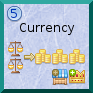
\includegraphics[scale=.7]{doe_tech_currency.png}
    \end{minipage}\hfill
    \begin{minipage}[c]{0.6\textwidth}
      \captionsetup{labelformat=empty, justification=justified, singlelinecheck=false}
      \caption{During your turn, you may convert 2 wealth to 3 money any number of times. Allows building of city improvement Market and wonder Tomb of Midas. (2)}
    \end{minipage}\hfill
    \label{fig:tech_currency}
  \end{figure}

  \begin{figure}[!htb]
    \begin{minipage}[c]{0.1\textwidth}
      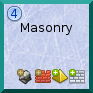
\includegraphics[scale=.7]{doe_tech_masonry.png}
    \end{minipage}\hfill
    \begin{minipage}[c]{0.6\textwidth}
      \captionsetup{labelformat=empty, justification=justified, singlelinecheck=false}
      \caption{Allows building of city improvements Workshop and Walls and wonders Pyramids and Great Wall. (3)}
    \end{minipage}\hfill
    \label{fig:tech_masonry}
  \end{figure}

  \begin{figure}[!htb]
    \begin{minipage}[c]{0.1\textwidth}
      
\includegraphics[scale=.7]{doe_tech_money_trade.png}
    \end{minipage}\hfill
    \begin{minipage}[c]{0.6\textwidth}
      \captionsetup{labelformat=empty, justification=justified, singlelinecheck=false}
      \caption{During your turn, you may convert 1 food to 1 money any number of times. Allows building of wonder Colossus. (1)}
    \end{minipage}\hfill
    \label{fig:tech_money_trade}
  \end{figure}

  \begin{figure}[!htb]
    \begin{minipage}[c]{0.1\textwidth}
      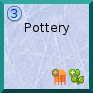
\includegraphics[scale=.7]{doe_tech_pottery.png}
    \end{minipage}\hfill
    \begin{minipage}[c]{0.6\textwidth}
      \captionsetup{labelformat=empty, justification=justified, singlelinecheck=false}
      \caption{Allows building of city improvement Granary and wonder Hanging Gardens. (2)}
    \end{minipage}\hfill
    \label{fig:tech_pottery}
  \end{figure}

  \begin{figure}[!htb]
    \begin{minipage}[c]{0.1\textwidth}
      
\includegraphics[scale=.7]{doe_tech_production_trade.png}
    \end{minipage}\hfill
    \begin{minipage}[c]{0.6\textwidth}
      \captionsetup{labelformat=empty, justification=justified, singlelinecheck=false}
      \caption{During your turn, you may convert 1 food to 1 production any number of times. Allows building of wonder Colossus. (1)}
    \end{minipage}\hfill
    \label{fig:tech_production_trade}
  \end{figure}

  \begin{figure}[!htb]
    \begin{minipage}[c]{0.1\textwidth}
      
\includegraphics[scale=.7]{doe_tech_science_trade.png}
    \end{minipage}\hfill
    \begin{minipage}[c]{0.6\textwidth}
      \captionsetup{labelformat=empty, justification=justified, singlelinecheck=false}
      \caption{During your turn, you may convert 1 food to 1 science any number of times. Allows building of wonder Colossus. (1)}
    \end{minipage}\hfill
    \label{fig:tech_science_trade}
  \end{figure}

  \begin{figure}[!htb]
    \begin{minipage}[c]{0.1\textwidth}
      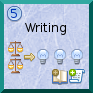
\includegraphics[scale=.7]{doe_tech_writing.png}
    \end{minipage}\hfill
    \begin{minipage}[c]{0.6\textwidth}
      \captionsetup{labelformat=empty, justification=justified, singlelinecheck=false}
      \caption{During your turn, you may convert 2 wealth to 3 science any number of times. Allows building of city improvement Library and wonder Great Library. (2)}
    \end{minipage}\hfill
    \label{fig:tech_writing}
  \end{figure}

  }\label{subsec:blue_technologies}
  \newpage
  \subsection{Yellow technologies}{

  \begin{figure}[!htb]
    \begin{minipage}[c]{0.1\textwidth}
      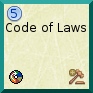
\includegraphics[scale=.7]{doe_tech_code_of_laws.png}
    \end{minipage}\hfill
    \begin{minipage}[c]{0.6\textwidth}
      \captionsetup{labelformat=empty, justification=justified, singlelinecheck=false}
      \caption{You may move one extra step in rondel. Allows building of city improvement Court. (2)}
    \end{minipage}\hfill
    \label{fig:tech_code_of_laws}
  \end{figure}

  \begin{figure}[!htb]
    \begin{minipage}[c]{0.1\textwidth}
      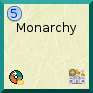
\includegraphics[scale=.7]{doe_tech_monarchy.png}
    \end{minipage}\hfill
    \begin{minipage}[c]{0.6\textwidth}
      \captionsetup{labelformat=empty, justification=justified, singlelinecheck=false}
      \caption{You may move extra steps in rondel by paying 1 money for each. Allows building of city improvement Palace. (3)}
    \end{minipage}\hfill
    \label{fig:tech_monarchy}
  \end{figure}

  \begin{figure}[!htb]
    \begin{minipage}[c]{0.1\textwidth}
      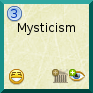
\includegraphics[scale=.7]{doe_tech_mysticism.png}
    \end{minipage}\hfill
    \begin{minipage}[c]{0.6\textwidth}
      \captionsetup{labelformat=empty, justification=justified, singlelinecheck=false}
      \caption{Provides 1 happy face. Allows building of city improvement Temple and wonder Oracle. (2)}
    \end{minipage}\hfill
    \label{fig:tech_mysticism}
  \end{figure}

  \begin{figure}[!htb]
    \begin{minipage}[c]{0.1\textwidth}
      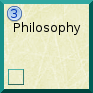
\includegraphics[scale=.7]{doe_tech_philosophy.png}
    \end{minipage}\hfill
    \begin{minipage}[c]{0.6\textwidth}
      \captionsetup{labelformat=empty, justification=justified, singlelinecheck=false}
      \caption{You may immediately take another technology tile by paying its cost. (1)}
    \end{minipage}\hfill
    \label{fig:tech_philosophy}
  \end{figure}

  \begin{figure}[!htb]
    \begin{minipage}[c]{0.1\textwidth}
      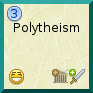
\includegraphics[scale=.7]{doe_tech_polytheism.png}
    \end{minipage}\hfill
    \begin{minipage}[c]{0.6\textwidth}
      \captionsetup{labelformat=empty, justification=justified, singlelinecheck=false}
      \caption{Provides 1 happy face. Allows building of city improvement Temple and wonder Temple of Mars. (2)}
    \end{minipage}\hfill
    \label{fig:tech_polytheism}
  \end{figure}

  \begin{figure}[!htb]
    \begin{minipage}[c]{0.1\textwidth}
      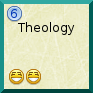
\includegraphics[scale=.7]{doe_tech_theology.png}
    \end{minipage}\hfill
    \begin{minipage}[c]{0.6\textwidth}
      \captionsetup{labelformat=empty, justification=justified, singlelinecheck=false}
      \caption{Provides 2 happy faces. (2)}
    \end{minipage}\hfill
    \label{fig:tech_theology}
  \end{figure}
  
  }\label{subsec:yellow_technologies}
  \newpage
  \subsection{Red technologies}{

    \begin{figure}[!htb]
    \begin{minipage}[c]{0.1\textwidth}
      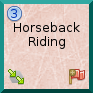
\includegraphics[scale=.7]{doe_tech_horseback_riding.png}
    \end{minipage}\hfill
    \begin{minipage}[c]{0.6\textwidth}
      \captionsetup{labelformat=empty, justification=justified, singlelinecheck=false}
      \caption{During movement, allows moving the same stack twice, provided that the first hex is not a mountain or ocean tile and has no enemies. Allows building of city improvement Barracks. (2)}
    \end{minipage}\hfill
    \label{fig:tech_horseback_riding}
  \end{figure}

  \begin{figure}[!htb]
    \begin{minipage}[c]{0.1\textwidth}
      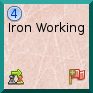
\includegraphics[scale=.7]{doe_tech_iron_working.png}
    \end{minipage}\hfill
    \begin{minipage}[c]{0.6\textwidth}
      \captionsetup{labelformat=empty, justification=justified, singlelinecheck=false}
      \caption{During movement, when attacking defender loses his warrior first instead of both warriors dying at the same time. Allows building of city improvement Barracks. (2)}
    \end{minipage}\hfill
    \label{fig:tech_iron_working}
  \end{figure}

  \begin{figure}[!htb]
    \begin{minipage}[c]{0.1\textwidth}
      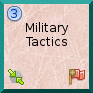
\includegraphics[scale=.7]{doe_tech_military_tactics.png}
    \end{minipage}\hfill
    \begin{minipage}[c]{0.6\textwidth}
      \captionsetup{labelformat=empty, justification=justified, singlelinecheck=false}
      \caption{During movement, allows movement of two separate stacks. Allows building of city improvement Barracks. (2)}
    \end{minipage}\hfill
    \label{fig:tech_military_tactics}
  \end{figure}

  \begin{figure}[!htb]
    \begin{minipage}[c]{0.1\textwidth}
      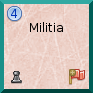
\includegraphics[scale=.7]{doe_tech_militia.png}
    \end{minipage}\hfill
    \begin{minipage}[c]{0.6\textwidth}
      \captionsetup{labelformat=empty, justification=justified, singlelinecheck=false}
      \caption{Gain an extra warrior and place it on your military upkeep track. Allows building of city improvement Barracks. (2)}
    \end{minipage}\hfill
    \label{fig:tech_militia}
  \end{figure}

  \begin{figure}[!htb]
    \begin{minipage}[c]{0.1\textwidth}
      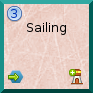
\includegraphics[scale=.7]{doe_tech_sailing.png}
    \end{minipage}\hfill
    \begin{minipage}[c]{0.6\textwidth}
      \captionsetup{labelformat=empty, justification=justified, singlelinecheck=false}
      \caption{During movement, allows movement to ocean tiles. Allows building of wonder Great Lighthouse. (4)}
    \end{minipage}\hfill
    \label{fig:tech_sailing}
  \end{figure}

  }\label{subsec:red_technologies}

}\label{sec:technology_tiles}

\newpage
\section{Appendix: City improvement tiles}{

  \begin{figure}[!htb]
    \begin{minipage}[c]{0.1\textwidth}
      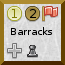
\includegraphics[scale=.7]{doe_building_barracks.png}
    \end{minipage}\hfill
    \begin{minipage}[c]{0.7\textwidth}
      \captionsetup{labelformat=empty, justification=justified, singlelinecheck=false}
      \caption{During recruit, allows building of an extra warrior. (4)}
    \end{minipage}\hfill
    \label{fig:building_barracks}
  \end{figure}

  \begin{figure}[!htb]
    \begin{minipage}[c]{0.1\textwidth}
      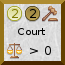
\includegraphics[scale=.7]{doe_building_court.png}
    \end{minipage}\hfill
    \begin{minipage}[c]{0.7\textwidth}
      \captionsetup{labelformat=empty, justification=justified, singlelinecheck=false}
      \caption{During harvest, you are allowed to store wealth. (2)}
    \end{minipage}\hfill
    \label{fig:building_court}
  \end{figure}

  \begin{figure}[!htb]
    \begin{minipage}[c]{0.1\textwidth}
      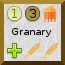
\includegraphics[scale=.7]{doe_building_granary.png}
    \end{minipage}\hfill
    \begin{minipage}[c]{0.7\textwidth}
      \captionsetup{labelformat=empty, justification=justified, singlelinecheck=false}
      \caption{During harvest, you gain 2 extra food. (2)}
    \end{minipage}\hfill
    \label{fig:building_granary}
  \end{figure}

  \begin{figure}[!htb]
    \begin{minipage}[c]{0.1\textwidth}
      
\includegraphics[scale=.7]{doe_building_library.png}
    \end{minipage}\hfill
    \begin{minipage}[c]{0.7\textwidth}
      \captionsetup{labelformat=empty, justification=justified, singlelinecheck=false}
      \caption{During harvest, you gain 2 extra science. (2)}
    \end{minipage}\hfill
    \label{fig:building_library}
  \end{figure}

  \begin{figure}[!htb]
    \begin{minipage}[c]{0.1\textwidth}
      
\includegraphics[scale=.7]{doe_building_market.png}
    \end{minipage}\hfill
    \begin{minipage}[c]{0.7\textwidth}
      \captionsetup{labelformat=empty, justification=justified, singlelinecheck=false}
      \caption{During harvest, you gain 2 extra money. (2)}
    \end{minipage}\hfill
    \label{fig:building_market}
  \end{figure}

  \begin{figure}[!htb]
    \begin{minipage}[c]{0.1\textwidth}
      
\includegraphics[scale=.7]{doe_building_palace.png}
    \end{minipage}\hfill
    \begin{minipage}[c]{0.7\textwidth}
      \captionsetup{labelformat=empty, justification=justified, singlelinecheck=false}
      \caption{Worth 1 victory point at the end of the game. (3)}
    \end{minipage}\hfill
    \label{fig:building_palace}
  \end{figure}

  \begin{figure}[!htb]
    \begin{minipage}[c]{0.1\textwidth}
      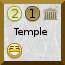
\includegraphics[scale=.7]{doe_building_temple.png}
    \end{minipage}\hfill
    \begin{minipage}[c]{0.7\textwidth}
      \captionsetup{labelformat=empty, justification=justified, singlelinecheck=false}
      \caption{Provides 1 happy face. (4)}
    \end{minipage}\hfill
    \label{fig:building_temple}
  \end{figure}

  \begin{figure}[!htb]
    \begin{minipage}[c]{0.1\textwidth}
      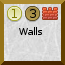
\includegraphics[scale=.7]{doe_building_walls.png}
    \end{minipage}\hfill
    \begin{minipage}[c]{0.7\textwidth}
      \captionsetup{labelformat=empty, justification=justified, singlelinecheck=false}
      \caption{Prevents opponents from entering your towns with a single warrior. (3)}
    \end{minipage}\hfill
    \label{fig:building_walls}
  \end{figure}

  \begin{figure}[!htb]
    \begin{minipage}[c]{0.1\textwidth}
      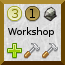
\includegraphics[scale=.7]{doe_building_workshop.png}
    \end{minipage}\hfill
    \begin{minipage}[c]{0.7\textwidth}
      \captionsetup{labelformat=empty, justification=justified, singlelinecheck=false}
      \caption{During harvest, you gain 2 extra production. (3)}
    \end{minipage}\hfill
    \label{fig:building_workshop}
  \end{figure}

}\label{sec:city_improvement_tiles}

\newpage
\section{Appendix: Wonder tiles}{

  \begin{figure}[!htb]
    \begin{minipage}[c]{0.1\textwidth}
      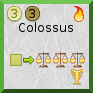
\includegraphics[scale=.7]{doe_wonder_colossus.png}
    \end{minipage}\hfill
    \begin{minipage}[c]{0.6\textwidth}
      \captionsetup{labelformat=empty, justification=justified, singlelinecheck=false}
      \caption{During harvest, you may convert cubes from plains to 3 wealth each. Worth 1 victory point at the end of the game.}
    \end{minipage}\hfill
    \label{fig:wonder_colossus}
  \end{figure}

  \begin{figure}[!htb]
    \begin{minipage}[c]{0.1\textwidth}
      
\includegraphics[scale=.7]{doe_wonder_great_library.png}
    \end{minipage}\hfill
    \begin{minipage}[c]{0.6\textwidth}
      \captionsetup{labelformat=empty, justification=justified, singlelinecheck=false}
      \caption{During your turn, you may convert 1 wealth to 2 science any number of times. Worth 1 victory point at the end of the game.}
    \end{minipage}\hfill
    \label{fig:wonder_great_library}
  \end{figure}

  \begin{figure}[!htb]
    \begin{minipage}[c]{0.1\textwidth}
      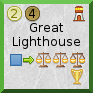
\includegraphics[scale=.7]{doe_wonder_great_lighthouse.png}
    \end{minipage}\hfill
    \begin{minipage}[c]{0.6\textwidth}
      \captionsetup{labelformat=empty, justification=justified, singlelinecheck=false}
      \caption{During harvest, you may convert cubes from ocean to 3 wealth each. Worth 1 victory point at the end of the game.}
    \end{minipage}\hfill
    \label{fig:wonder_great_lighthouse}
  \end{figure}

  \begin{figure}[!htb]
    \begin{minipage}[c]{0.1\textwidth}
      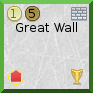
\includegraphics[scale=.7]{doe_wonder_great_wall.png}
    \end{minipage}\hfill
    \begin{minipage}[c]{0.6\textwidth}
      \captionsetup{labelformat=empty, justification=justified, singlelinecheck=false}
      \caption{Prevents opponents from entering your towns completely. Worth 1 victory point at the end of the game.}
    \end{minipage}\hfill
    \label{fig:wonder_great_wall}
  \end{figure}

  \begin{figure}[!htb]
    \begin{minipage}[c]{0.1\textwidth}
      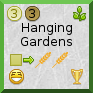
\includegraphics[scale=.7]{doe_wonder_hanging_gardens.png}
    \end{minipage}\hfill
    \begin{minipage}[c]{0.6\textwidth}
      \captionsetup{labelformat=empty, justification=justified, singlelinecheck=false}
      \caption{During harvest, you may convert cubes from plains to 2 food each. Provides 1 happy face. Worth 1 victory point at the end of the game.}
    \end{minipage}\hfill
    \label{fig:wonder_hanging_gardens}
  \end{figure}

  \begin{figure}[!htb]
    \begin{minipage}[c]{0.1\textwidth}
      \includegraphics[scale=.7]{doe_wonder_oracle.png}
    \end{minipage}\hfill
    \begin{minipage}[c]{0.6\textwidth}
      \captionsetup{labelformat=empty, justification=justified, singlelinecheck=false}
      \caption{Provides 2 happy faces. Worth 1 victory point at the end of the game.}
    \end{minipage}\hfill
    \label{fig:wonder_oracle}
  \end{figure}

  \begin{figure}[!htb]
    \begin{minipage}[c]{0.1\textwidth}
      \includegraphics[scale=.7]{doe_wonder_pyramids.png}
    \end{minipage}\hfill
    \begin{minipage}[c]{0.6\textwidth}
      \captionsetup{labelformat=empty, justification=justified, singlelinecheck=false}
      \caption{During harvest, you may convert cubes from desert to 2 food each. Worth 2 victory points at the end of the game.}
    \end{minipage}\hfill
    \label{fig:wonder_pyramids}
  \end{figure}

  \begin{figure}[!htb]
    \begin{minipage}[c]{0.1\textwidth}
      \includegraphics[scale=.7]{doe_wonder_temple_of_mars.png}
    \end{minipage}\hfill
    \begin{minipage}[c]{0.6\textwidth}
      \captionsetup{labelformat=empty, justification=justified, singlelinecheck=false}
      \caption{Place white warrior (Spirit of Mars) to an empty tile adjacent
        to any of your towns and see Section Spirit of Mars for more details.
        Worth 1 victory point at end of the game per each two empty spaces on military upkeep track.}
    \end{minipage}\hfill
    \label{fig:wonder_temple_of_mars}
  \end{figure}

  \begin{figure}[!htb]
    \begin{minipage}[c]{0.1\textwidth}
      \includegraphics[scale=.7]{doe_wonder_tomb_of_midas.png}
    \end{minipage}\hfill
    \begin{minipage}[c]{0.6\textwidth}
      \captionsetup{labelformat=empty, justification=justified, singlelinecheck=false}
      \caption{During your turn, you may convert 1 wealth to 2 money any number of times. Worth 1 victory point at the end of the game.}
    \end{minipage}\hfill
    \label{fig:wonder_tomb_of_midas}
  \end{figure}

}\label{sec:wonder_tiles}

\end{document}
